\section{\glsentryshort{pws} Dynamical Systems}
\label{sec:state.discont}

Initially, the theory of non-linear dynamical systems was developed for smooth dynamical systems only.
Hence, several results can't be applied to \gls{pws} dynamical systems.
But smooth systems are not fit to model several engineering applications, since such systems often undergo sudden changes.
For example, a model of an electrical circuit can't be smooth as soon as the circuit has a single switching element, such as a transistor~\cite{ZhuMos03}.
The model we will investigate in this thesis describes such an electrical circuit.

In \gls{pws} dynamical systems, bifurcations are possible, that do not occur in smooth dynamical systems.
Even more so in \gls{pws} discontinuous dynamical systems, which this thesis focuses on.
While the theory for continuous-time 1D \gls{pws} discontinuous dynamical systems is quite complete, the theory for time-discrete 1D \gls{pws} discontinuous dynamical systems in is further behind~\cite{Simpson16}.
Also while in smooth dynamical systems and \gls{pws} continuous dynamical systems bifurcations can be generalized and described using normal forms, this is not possible for \gls{pws} discontinuous dynamical systems.
The reason for this is that many bifurcations, especially \glspl{bcb}, are necessarily global and normal forms only work for local bifurcations.
\todo{citation}
The advantage of normal forms is that these models neglect all non-essential parameter effects for the description of the bifurcation phenomenon at hand.
Furthermore, one can prove that the neglected parameter effects are indeed non-essential for the bifurcation phenomenon.
For the model considered in this thesis, such a proof can not be provided.
Nevertheless, we will follow a similar approach as we will neglect parameter effects, we identify as non-essential.
But rather than on rigorous proofs, we rely on numerical evidence.
We will call the resulting model an archetypal model.

The bifurcations covered in this thesis all belong to the previously mentioned class of \glspl{bcb}.

\begin{definition}[Border Collision]
	A \glsentrylong{bc} is a point in the parameter space, where an invariant set (e.g a fixed point or a cycle) collides with a border of the model function in the state space.
\end{definition}

Note that the \hl{points} of the state space, where the model function is not smooth are called borders.

\begin{definition}[Border Collision Bifurcation]
	A \glsentrylong{bcb} is a \gls{bc} that also causes a qualitative change in the state space topology.
\end{definition}

Since model functions of \gls{pws} dynamical systems consist of multiple branches, we can describe cycles in such systems using symbolic sequences.
This allows us to differentiate between different cycles even if they have the same period.

\begin{definition}[Symbolic Sequence]
	Let $f: \mathbb{R} \to \mathbb{R}$ be the model function of a \gls{pws} dynamical system that is divided into $n$ partitions $I_j$ where $0 \leq j < n$.
	Let the set of symbols associated with each partition $I_j$ be $\left\{S_j\right\}_{0 \leq j < n}$.
	The symbolic sequence $S_f(\O_k)$ of a cycle $\O_k = \left\{x_i \:\mid\: 0 \leq i < k\right\}$ is defined in the following way.
	\begin{align}
		S_f(\O_k) = \left(o(x_0), o(x_1), \dots, o(x_{k-1})\right)
	\end{align}
	Where the function $o$ provides a symbol for every point of the cycle.
	It is defined as $o(x) = S_j$ if $x \in S_j$ for all $0 \leq j < n$~\cite{granados14adding}.
\end{definition}

For example, a $k$-cycle in a \gls{pws} dynamical system divided into two partitions $I_0 = \left\{x \:\mid\: x < 0\right\}$ and $I_1 = \left\{x \:\mid\: x > 0\right\}$ with symbols $S_0 = \L$ and $S_1 = \R$ that has one point $x_0 \in I_0$ and $k-1$ points $x_j \in I_1, \:1 \leq j < k$ is associated with the symbolic sequence $\L\R^{k-1}$.
\todo{Picture of such a cycle}

We will now introduce a class of bifurcation structures that this thesis covers towards the end in \Cref{chap:add}.
Bifurcation structures belonging to this class called period-adding structures can be found in many \gls{pws} dynamical systems.

Period-adding structures are named like this because in such structures, between a parameter region with a cycle of period $a$ and another parameter region with a cycle of period $b$, there is a parameter region with a cycle of period $a + b$.

\begin{figure}
	\centering
	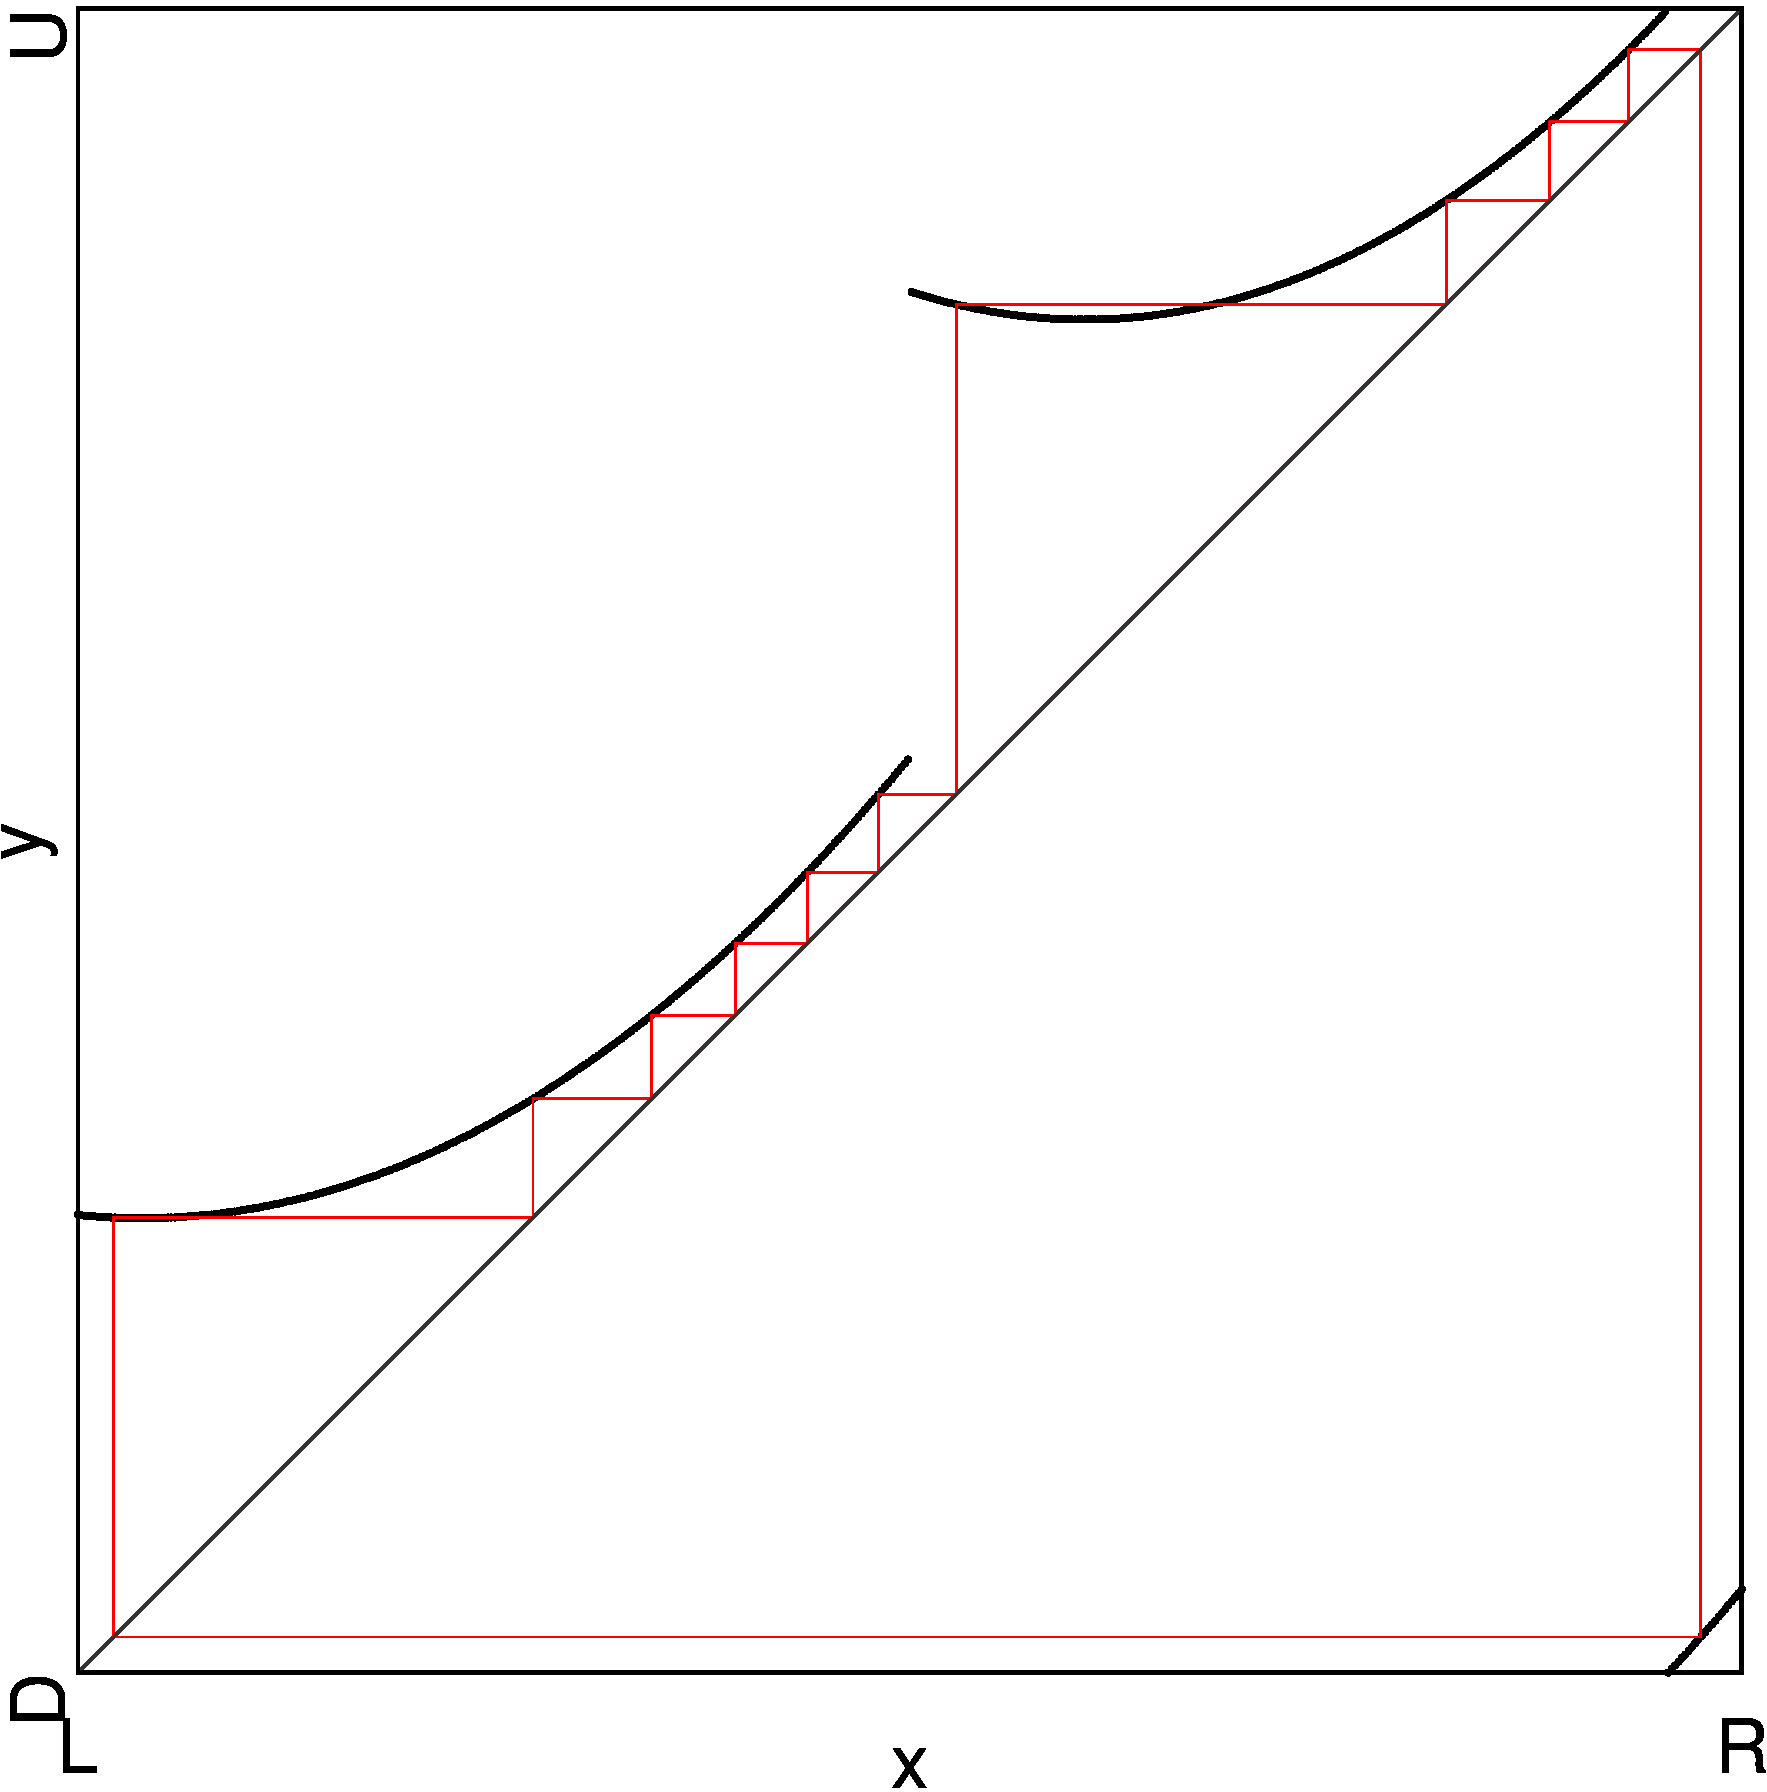
\includegraphics[width=.5 \textwidth]{80_Adding_LR/1D_Period/result.png}
	\caption[1D scan of periods in a period-adding structure between $\L$ and $\R$]{
		1D scan of the periods of cycles in a period-adding structure with the starting cycles $\L$ and $\R$.
	}
\end{figure}

An even more compact way to differentiate between multiple cycles that have the same period are rotation number.
Here, we will use them to describe the structure of period-adding structures.

\begin{definition}[Rotation Numbers --- Keener]
	Let $\sigma$ be a cycle of a \gls{pws} dynamical system $x_{n+1} = f(x_n)$ with two branches, $\L$ and $\R$.
	Then the rotation number $\rho(\sigma)$ of this cycle is defined as the ratio of number of letters $\L$ in the symbolic sequence of the cycle divided by the period of the cycle $\sigma$~\cite{Keener80}.
	\begin{align}
		\rho(\sigma) = \dfrac{|\sigma|_\L}{|\sigma|}
	\end{align}
\end{definition}

The rotation numbers of the cycles in a period-adding structure are organized in a Farey-tree.
A Farey-tree has two ``root nodes'' and the child node of two nodes is the Farey-sum of the parent nodes~\cite{granados14adding}.

\begin{definition}[Farey-sum]
	The Farey-sum $a \oplus b$ of two fractions $a = \frac{a_1}{a_2}$ and $b = \frac{b_1}{b_2}$ is defined in the following way.
	\begin{align}
		a \oplus b = \frac{a_1}{a_2} \oplus \frac{b_1}{b_2} = \dfrac{a_1 + b_1}{a_2 + b_2}
	\end{align}
\end{definition}

\Cref{fig:state.discont.adding.farey.rot} shows such a Farey-tree of a period-adding structure between two fixed points, $\L$ and $\R$.
If we replace the content of the nodes with the symbolic sequences of the cycles, we get the tree shown in \Cref{fig:state.discont.adding.farey.rot}.
Instead of Farey-addition, here the child node of two parent nodes is the concatenation of the symbolic sequences in the parent nodes.
Together with \Cref{theorem:state.rot.num.concat}, this explains why the  tree in \Cref{fig:state.discont.adding.farey.rot} is a Farey-tree~\cite{granados14adding}.

\begin{theorem}[Rotation Numbers of Concatenated Cycles]
	The rotation number of the concatenation of two cycles $\rho(\sigma\varrho)$ is the Farey-sum of the rotation numbers of both cycles, $\rho(\sigma) \oplus \rho(\varrho)$.
	\label{theorem:state.rot.num.concat}
\end{theorem}

\begin{proof}
	\begin{align*}
		\rho(\sigma\varrho)
		= \dfrac{|\sigma\varrho|_\L}{|\sigma\varrho|}
		= \dfrac{|\sigma|_\L + |\varrho|_\L}{|\sigma| + |\varrho|}
		= \dfrac{|\sigma|_\L}{|\sigma|} \oplus \dfrac{|\varrho|_\L}{|\varrho|}
		= \rho(\sigma) \oplus \rho(\varrho)
	\end{align*}
	\vspace{-4.8em}
	\begin{flushright}
		$\blacksquare$
	\end{flushright}
\end{proof}

\begin{figure}
	\centering
	\subfloat[Rotation Numbers]{
		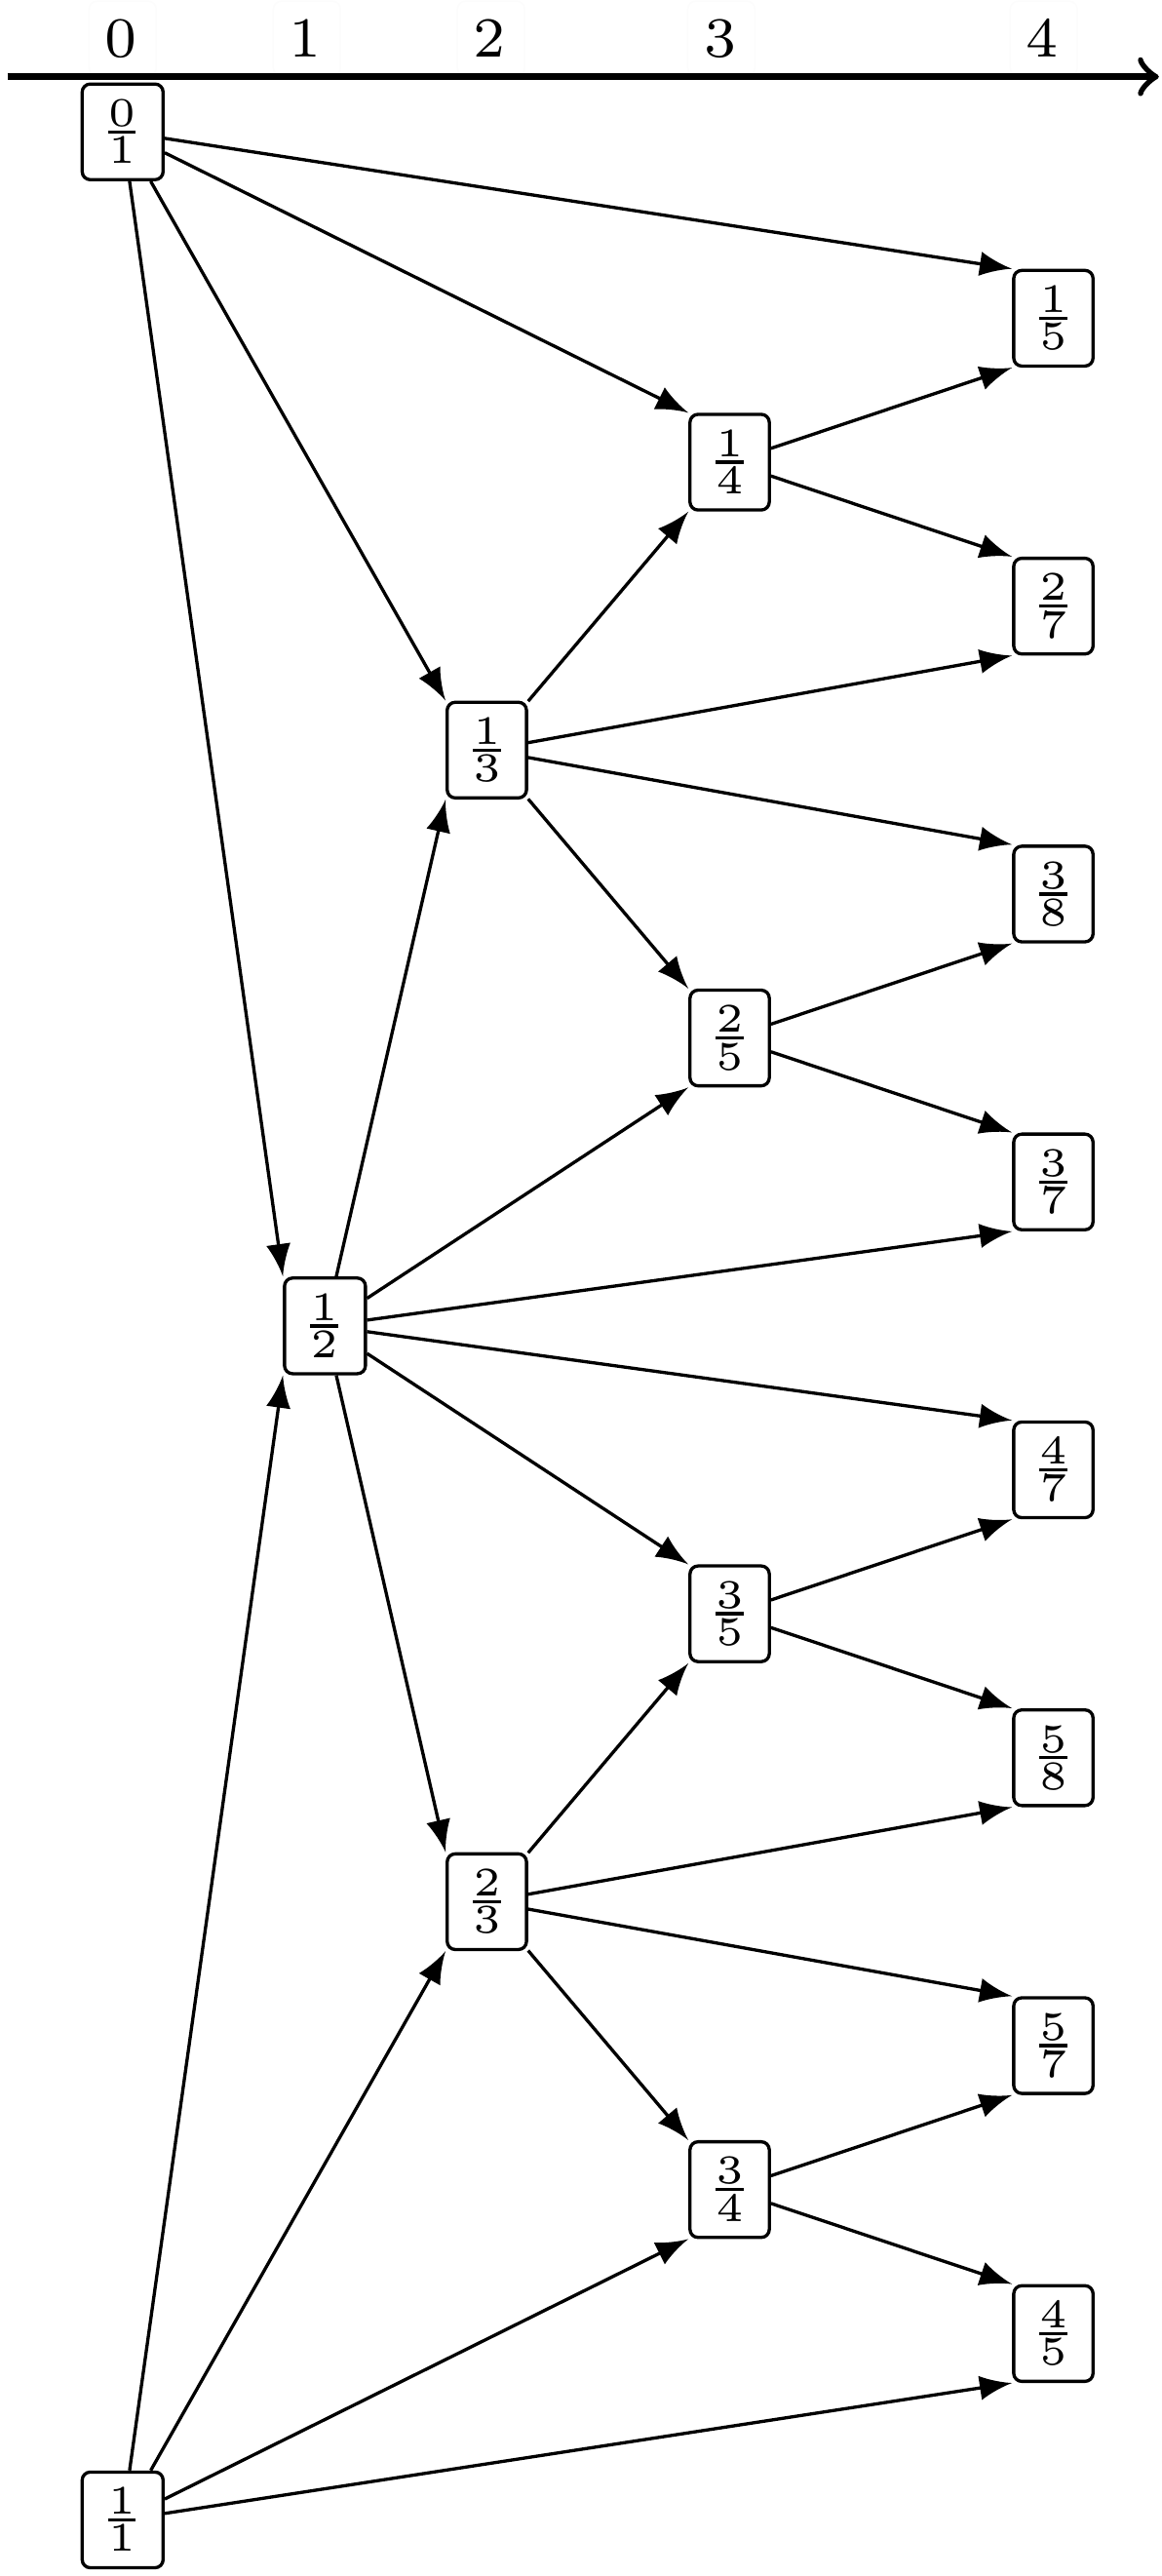
\includegraphics[height=.4 \textheight]{Figures/FareyTrees/LR_RotNum/adding.png}
		\label{fig:state.discont.adding.farey.rot}
	}
	\quad
	\subfloat[Symbolic Sequences]{
		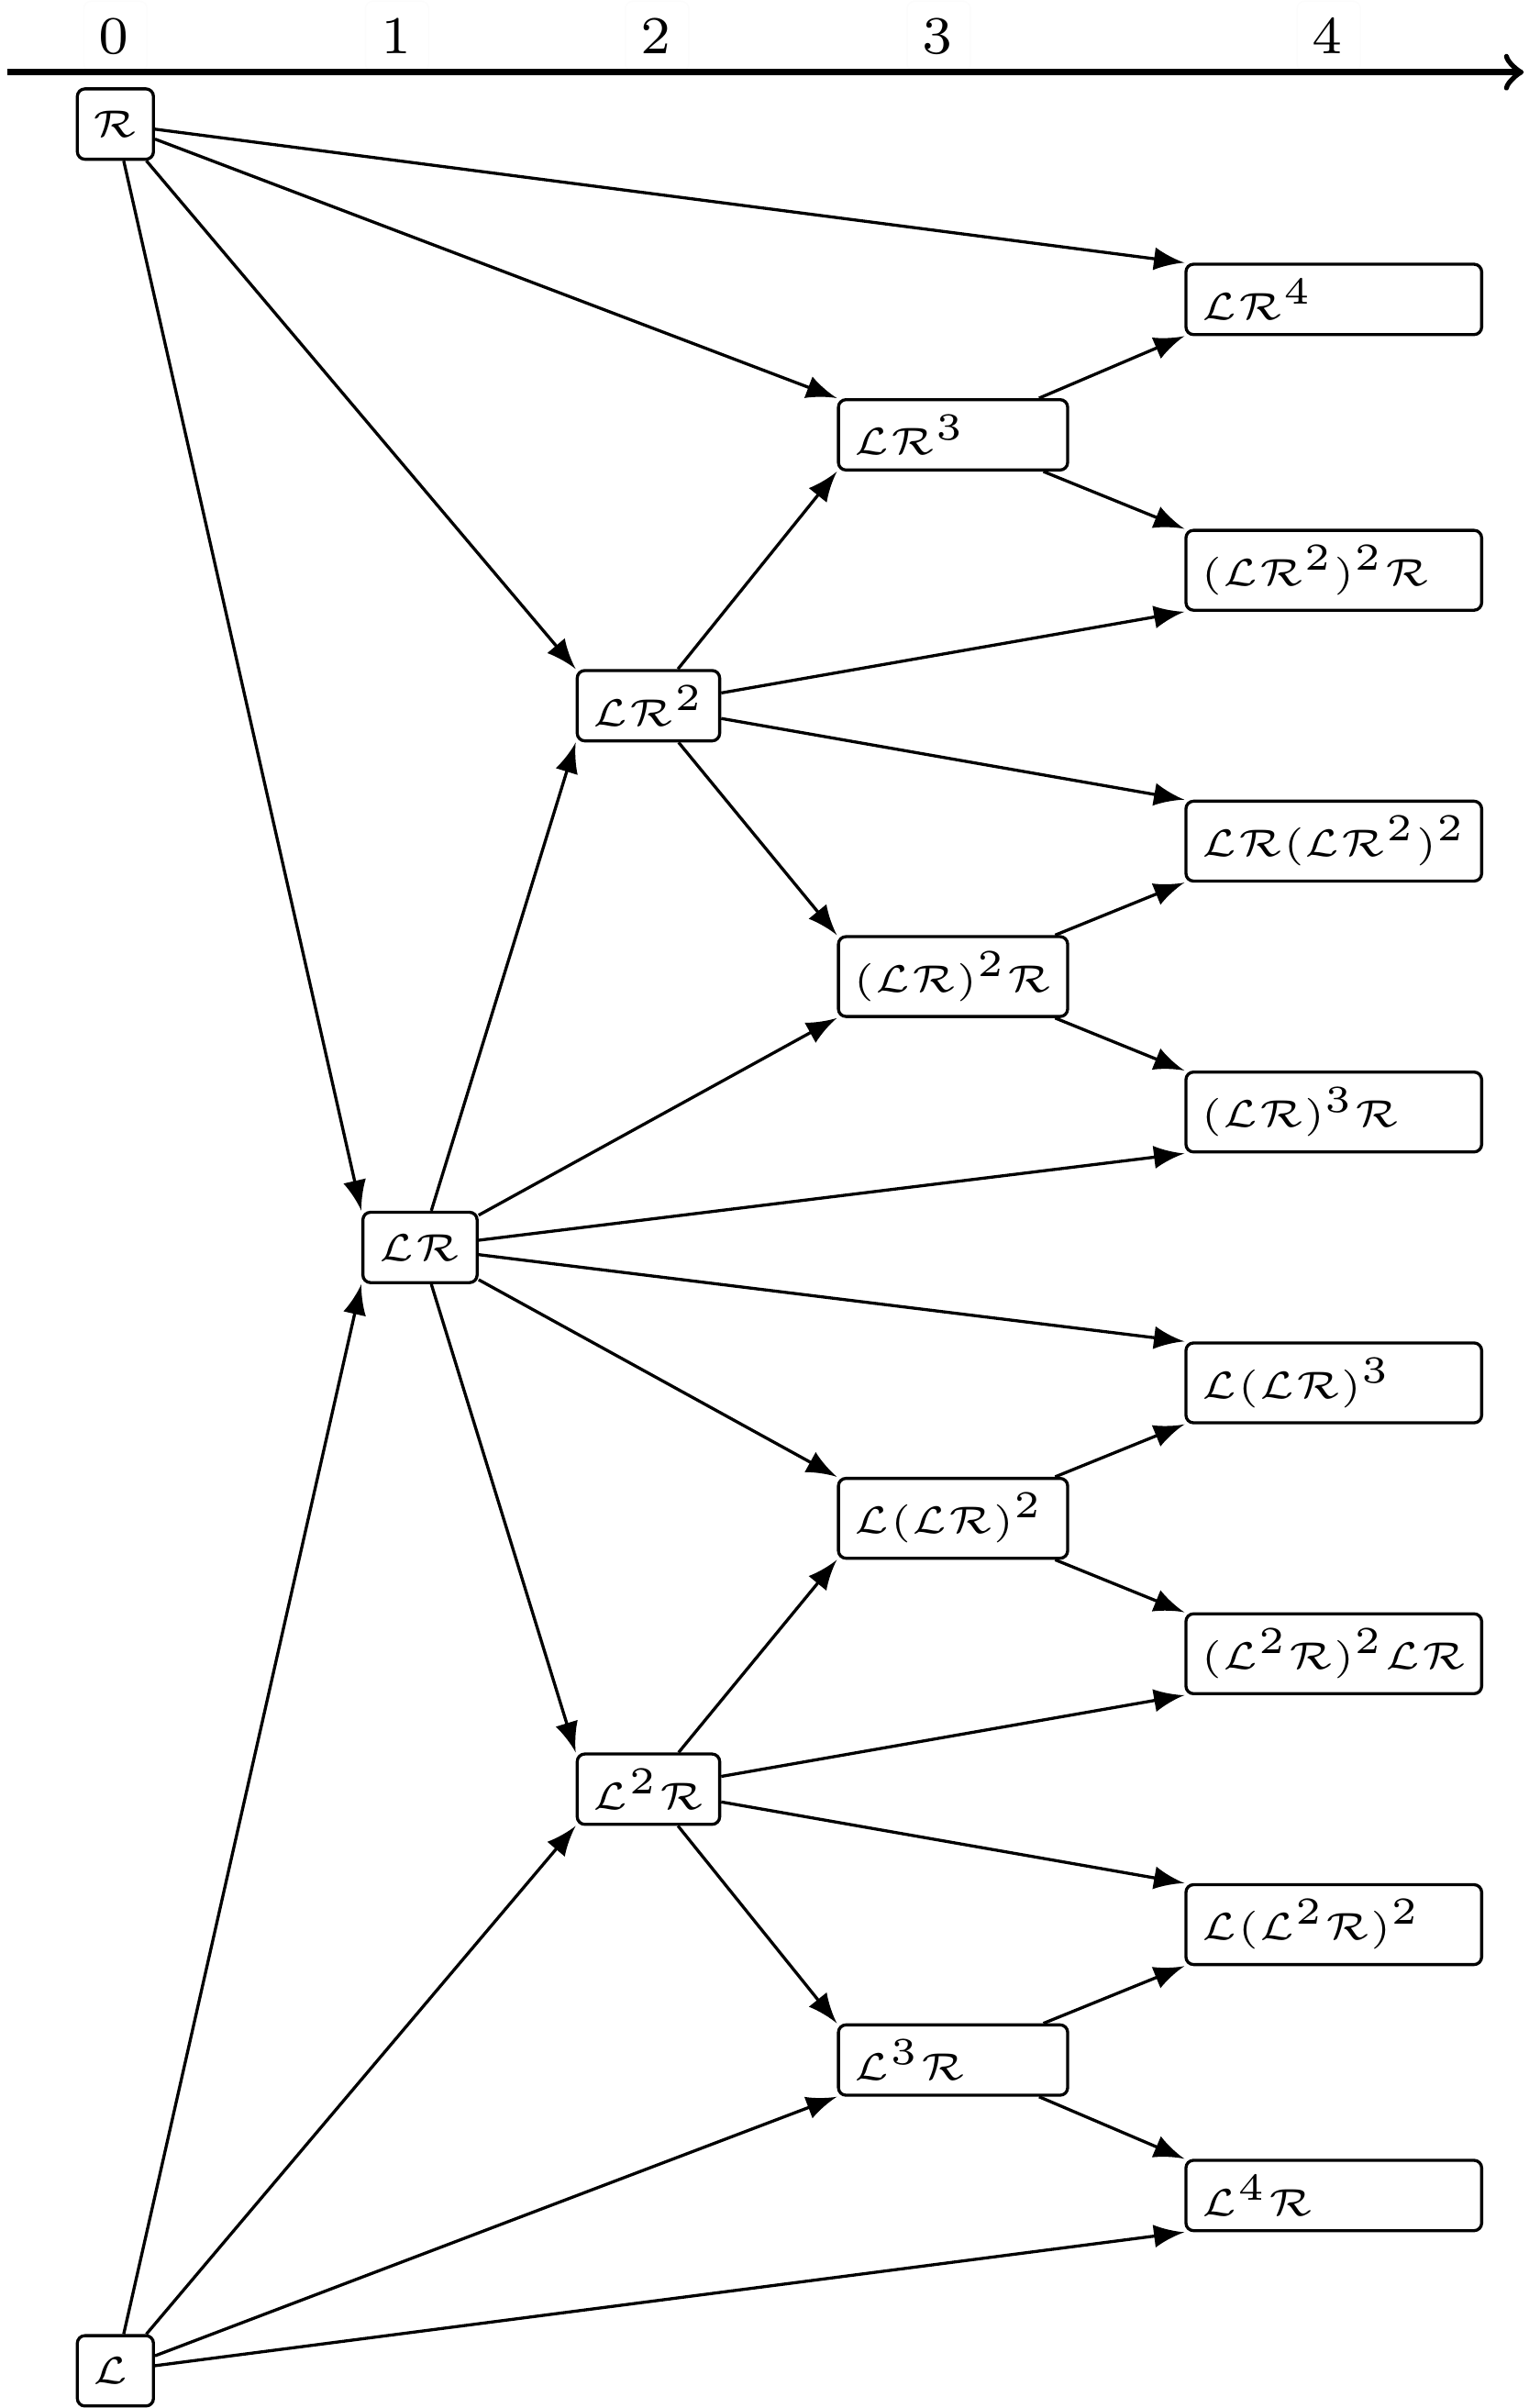
\includegraphics[height=.4 \textheight]{Figures/FareyTrees/LR/adding.png}
		\label{fig:state.discont.adding.farey.sym}
	}
	\caption[Farey-trees of a period-adding structure between $\L$ and $\R$]{
		Farey-trees of a period-adding structure with the starting cycles $\L$ and $\R$.
		(a) Shows the rotation numbers while (b) shows the symbolic sequences of the cycles in this structure.
	}
	\label{fig:state.discont.adding.farey}
\end{figure}
